\subsection{RESTful API}
La RESTful API fue diseñada en primera instancia durante el cursado de la materia Laboratorio de programación utilizando JavaScript, Node.js y Express.js. Para la implementación de este trabajo se realizo una nueva API usando las mismas tecnologías y tomando como base la anterior mencionada con el fin de mejorar aspectos organizativos y funcionales.

Ademas con el fin de tener información persistente se agrego una base de datos mySQL para el almacenamiento de la información, considerando que las imágenes a utilizar iban a ser cargadas en un almacenamiento en la nube por lo que solo es necesario almacenar el enlace a estas para poder accederlas luego.

\begin{figure}[!h]
  \centering
  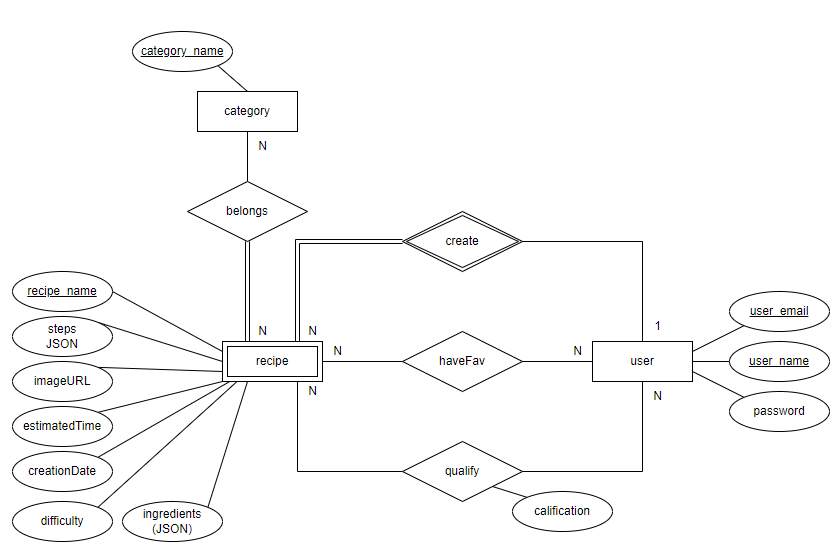
\includegraphics[width=16cm, scale=1]{Images/Imagenes/MER.png}
  \caption{Modelo entidad relación de la base de datos implementada}
  \label{fig:marcado}
\end{figure}

La implementación cuenta con método de población de la base de datos que puede ser ejecutado con el comando  \texttt{npm run populate}. Este se encargara de cargar con usuarios, recetas, categorías y favoritos a la base de datos para agilizar su prueba.

\subsection{Patrón MVC}
Como patron de diseño para la implementacion se utilizo Model View Controller (MVC). Este consiste en las siguientes capas:
\begin{itemize}
  \item \textbf{El modelo: }Representa los datos y la lógica de negocio de la aplicación. En el caso de esta implementación se corresponde con la capa de servicios que se encarga de realizar las consultas a la base de datos de forma directa. Puede encontrarse en el directorio \texttt{/services}
  \item \textbf{La vista: }Es la capa de presentación de la aplicación, que se encarga de mostrar los datos al usuario. En el contexto de una API RESTful, esta capa se corresponde con las respuestas que envía el servidor a las peticiones realizadas por los clientes. Puede encontrarse en el directorio \texttt{/routes}
  \item \textbf{El controlador: }es la capa que se encarga de manejar las peticiones del usuario, interactuar con el modelo para obtener los datos necesarios y devolver la respuesta adecuada. En este caso se utilizaron rutas y controladores que reciben peticiones, validan los datos y solicitan informacion a los servicios correspondientes. Puede encontrarse en los directorios \texttt{/controllers} y \texttt{/middlewares/validators}
\end{itemize}

\subsection{Ejecución Otras consideraciones}
Una vez configurado el .env de manera adecuada la API puede ponerse en marcha con el comando \texttt{npm run dev}.

Otras bibliotecas importantes para la implementación de la api son:

\begin{itemize}
  \item \textbf{Bcrypt: }Para realizar el cifrado de las contraseñas de los usuarios
  \item \textbf{Dotenv: }Para definir variables de entorno y facilitar asi la configuración de la API y la base de datos. Es conveniente revisar dicho archivo para configurar adecuadamente la API e iniciar la ejecución.  
  \item \textbf{JSON Web Token (JWT): }como mecanismo de autenticación y autorización con los clientes
\end{itemize}

Para el realizar pruebas se hizo uso de Postman, en la figura [\ref{fig:postman}] se puede observar la lista de pruebas realizadas las cuales también se corresponden con los diferentes servicios que brinda la API.

\begin{figure}[!htb]
  \centering
  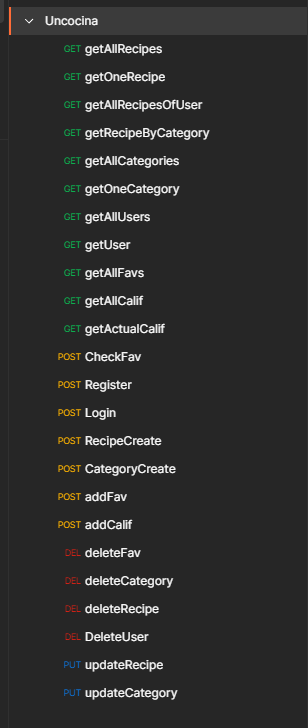
\includegraphics[width=8cm, scale=1]{Images/Imagenes/postman.png}
  \caption{Lista de pruebas realizadas a la API con Postman}
  \label{fig:postman}
\end{figure}

